\chapter{Referencial Teórico}
\label{cap:ref-teorico}
Neste capítulo serão apresentados os fundamentos pertinentes a este trabalho. A Seção \ref{ref-teo:npm} apresenta o conceito e o funcionamento do \gls{NPM} bem como a questão das dependências. A Seção \ref{ref-teo:prov_clie} distingue os termos \textit{provedor} e \textit{cliente}. Também para diferenciar termos, a Seção \ref{ref-teo:pac_rel_ver} conceitua as palavras \textit{pacote}, \textit{release} e \textit{versão}. Já na Seção \ref{ref-teo:node}, é explicado o conceito do \textit{Node.js}. A Seção \ref{ref-teo:semver} explica o que é o \textit{Semantic Versioning}, o \textit{SemVer} e como eles são utilizados no ecossistema do \gls{NPM}. Porfim, a Seção \ref{ref-teo:breaking_change} conceitua e exemplifica as \textit{breaking changes}.

\section{\gls{NPM}}
\label{ref-teo:npm}
O \gls{NPM} é um gerenciador de pacotes para o \textit{Node.js}. Lançado em 2009, seu principal objetivo é facilitar o compartilhamento de códigos escritos em \textit{Javascript}. Atualmente, o \gls{NPM} ocupa a posição de maior repositório para uma dada linguagem, com mais de 1 milhão de projetos\footnote{http://www.modulecounts.com/}. O \gls{NPM} permite que, com apenas um simples comando, o usuário realize o download, publique, instale e desinstale pacotes diretamente do repositório. A facilidade proporcionada pelo \gls{NPM} corrobora para a grande popularidade do \textit{Javascript} e para que o compartilhamento de biblioteca seja largamente utilizado, uma vez que 97\% dos aplicativos \textit{web} são oriundos do \textit{NPM}\footnote{https://blog.npmjs.org/post/180868064080/this-year-in-javascript-2018-in-review-and-npms}.

O ecossistema \gls{NPM} estimula o compartilhamento de código entre aos pacotes. Por causa disso, o \gls{NPM}, dentre os demais repositórios, contém a maior distribuição de dependência entre os pacotes \cite{teorical_reference:npm_2}. Desta maneira, como muitos pacotes estão dependendo mutuamente uns dos outros, há uma gigantesca rede de interconectividade entre os pacotes. Entretanto, quando há um erro qualquer em algum destes pacotes, um grande número de outros pacotes podem ser afetados. Foi exatamente isso que ocorreu com um pacote chamado \textit{left-pad}\footnote{https://blog.npmjs.org/post/141577284765/kik-left-pad-and-npm}. Este pacote foi removido do \textit{NPM} por seu desenvolvedor e impactou milhares de pacotes em apenas 2.5 horas incluindo pacotes renomados como o \textit{babel}\footnote{https://github.com/babel/babel} e o \textit{atom}\footnote{https://github.com/atom/atom} que, devido ao grande número de dependentes, cascatearam o erro para inúmeros outros pacotes.
%In fact, 97\% of the code in a modern web application comes from npm

\section{Provedor e Cliente}
\label{ref-teo:prov_clie}
O pacote provedor é aquele que provê recursos ao pacote cliente, ou seja, contém interfaces públicas para acesso às suas funcionalidades. O termo \textit{pacote provedor} pode ser interpretado como \textit{bibliotecas} ou \textit{dependências}. É do provedor que emana a responsabilidade de indicar o nível de compatibilidade que sua nova \textit{release} está introduzindo \cite{teorical_reference:semver}. Por exemplo, quando é executado o seguinte comando

\begin{lstlisting}[style=bash, label=cod:install:provider]
npm install any_package
\end{lstlisting}
o \gls{NPM} salva o \textit{any\_package} no \textit{package.json} como uma dependência. Nesse momento, o \textit{any\_package} se torna um pacote provedor. Assim, o pacote \textit{any\_package} é um provedor direto, pois foi instalado diretamente pelo usuário. Entretanto, as dependências do \textit{any\_package} também são instaladas, mas de forma indireta pelo \gls{NPM}. Estes outros pacotes são chamados de \textit{provedores indiretos}, pois não dependem que o usuário instale-os diretamente com o comando \textit{npm install}.

Já o pacote cliente é aquele que está acessando as interfaces públicas do provedor. Quando uma \textit{break change} é introduzida pelo provedor -- direto ou indireto --, é sempre no pacote cliente que esta \textit{break change} se manifesta, causando o encerramento da execução. O pacote cliente é aquele que possui a responsabilidade de atualizar a versão de seus provedores no \textit{package.json} quando esses publicam uma \textit{release} com correções.

\section{Pacote, \textit{Release} e Versão}
\label{ref-teo:pac_rel_ver}
Neste artigo, a palavra \textit{pacote} refere-se a um \textit{software} hospedado no \gls{NPM}. Este \textit{software} contém seu nome, seus arquivos e suas versões. Por exemplo, quando nos referimos ao pacote \textit{mocha}, nos referimos à ideia genérica deste pacote, sem levar em consideração uma versão específica ou seu estado em algum instante, mas sim, apenas ao pacote como um todo.

Já a palavra \textit{release} designa o estado de um pacote em um determinado instante. uma \textit{release} é denotada por uma versão específica deste pacote, isto é, um conjunto de arquivos distintos das demais \textit{releases}. Cada \textit{release} é acompanhada da publicação de uma nova versão do pacote no \gls{NPM}.

Por fim, o termo \textit{versão} é utilizado para especificar e distinguir um determinado estado de uma \textit{release}. Uma \textit{versão} é uma \textit{string} no padrão \gls{SemVer} que identifica unicamente uma determinada \textit{release} e é utilizada pelo \gls{NPM} no arquivo \textit{package.json} para especificar um \textit{range} de versões que o cliente aceita.

\section{Node.js}
\label{ref-teo:node}
O \textit{Node.js} é um projeto \textit{open-source} implementado em \textit{C++} sobre a \textit{engine Javascript V8} do \textit{Google}, que é um compilador \textit{Javascript} para \textit{web}. O \textit{Node.js} foi criado com o objetivo de estender o código \textit{Javascript} para além do \textit{front-end} de forma que o \textit{Javascript} possa ser executado no \textit{back-end} também. Com o \textit{Javascript} executando no \textit{front-end} e no \textit{back-end} não se faz necessário que os desenvolvedores saibam duas linguagens de programação diferentes. A utilização do \textit{Javascript} no \textit{front} e no \textit{back-end}, através do \textit{Node.js}, foi um dos principais fatores que levou à grande popularidade do \textit{Javascript}, uma vez que o \textit{Node.js} é o \textit{framework} mais utilizado atualmente, de acordo com o \textit{Stack Overflow}\footnote{https://insights.stackoverflow.com/survey/2019\#technology-\_-other-frameworks-libraries-and-tools}.

\section{\gls{SemVer}}
\label{ref-teo:semver}
O \gls{SemVer}\footnote{https://semver.org} é um padrão para versionamento de \textit{releases} de um projeto a partir do tipo de alteração introduzida na \textit{release}. Com o \gls{SemVer} é possível evoluir um projeto sempre mantendo a compatibilidade com versões anteriores através de um \textit{range de versões} na qual está especificada uma determinada versão. O padrão \gls{SemVer} é largamente utilizada no desenvolvimento de projetos. As regras do \gls{SemVer} foram idealizadas por Tom Preston-Werner -- criador do \textit{GitHub} -- que incentiva todos os desenvolvedores à utilizarem este padrão, uma vez que as regras são baseadas em práticas comuns já utilizadas em projetos \cite{teorical_reference:semver}.

O esquema de versionamento, basicamente, é uma \textit{string} que possui três dígitos: \textit{major.minor.path}. Os dígitos do \gls{SemVer} devem ser incrementados de acordo com o tipo de alteração que a \textit{release} do projeto está introduzindo. O número \textit{major} deve ser incrementado quando uma \textit{release} introduz \textit{breaking changes}; o \textit{minor}, quando é adicionada melhorias/novas funcionalidades que mantenham a compatibilidade com as \textit{releases} anteriores; e o \textit{path}, quando a \textit{release} contém correção de \textit{bugs}. Com a padronização do \gls{SemVer} é possível que os desenvolvedores introduzem \textit{breaking changes} sem que essas afetem os clientes, uma vez que, por meio da \textit{string} de versionamento, eles não receberão a \textit{release} com \textit{breaking changes}.

O \gls{NPM} utiliza o padrão \gls{SemVer} no arquivo \textit{package.json} -- arquivo de configuração do projeto que contém todas as suas dependências e suas respectivas versões. Ao executar o comando \textit{npm install express --save}, para instalar a dependência \textit{express}\footnote{https://www.npmjs.com/package/express} por exemplo, o \gls{NPM} -- além de descarregar essa dependência -- irá salvar no \textit{package.json} o nome dessa dependência com sua versão atual em modo \textit{range}, de acordo com a Figura \ref{fig:dep_express}.

\begin{figure}
    \centering
    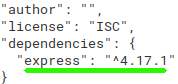
\includegraphics{figuras/dependencies_express.png}
    \caption{Modo como o \gls{NPM} salva no \textit{package.json} a versão de uma dependência}
    \label{fig:dep_express}
\end{figure}{}

Com a informação da versão da dependência no \textit{package.json}, o cliente não precisa se preocupar com as novas atualizações de sua dependência, uma vez que o \gls{NPM}, ao instalar novamente as dependências, sempre irá descarregar a \textit{release} mais recente da dependência que não contenha uma \textit{breaking change}, ou seja, a última \textit{release} disponível para a mesma versão \textit{major} -- desde que a \textit{string} de versionamento seja salva em modo \textit{range} (\textasciicircum).

\section{Breaking Change}
\label{ref-teo:breaking_change}
Uma \textit{break change} é uma alteração no pacote provedor que produz defeitos nos pacotes clientes \cite{teorical_reference:semver}. Para evitar que os impactos de uma \textit{break change} afetem os clientes, os provedores publicam suas \textit{releases} com \textit{breaking changes} incrementando o nível \textit{major} do \gls{SemVer}. Desta maneira, os clientes de versões prévias não serão afetados.

Durante o desenvolvimento de \textit{software}, os provedores precisam introduzir \textit{breaking changes}, pois quando só há \textit{releases} compatíveis com versões anteriores, os pacotes perdem muitas oportunidades de evolução \cite{teorical_reference:bc_2}. Desta maneira, as \textit{break changes} são importantes para a evolução de um \textit{software}, uma vez que apenas \textit{releases} retro-compatíveis podem estagnar o \textit{software} limitando sua evolução. Assim, as \textit{breaking changes} também são sinônimos de evolução. Exemplo disso é o \textit{Node.js} que publica uma \textit{release} incrementando o nível \textit{major} a cada 6 meses\footnote{https://github.com/nodejs/node\#release-types}. Desta maneira, introduzir \textit{breaking changes} em níveis \textit{major} permite que os \textit{softwares} evoluam sem manter-se preso à versões anteriores e evita que esta \textit{breaking change} afete o cliente -- desde que o \textit{range} do provedor esteja especificado para o \textit{range carret} ou \textit{tilde}.

Uma \textit{breaking change} pode ser introduzida em uma \textit{release} intencionalmente -- quando é atualizada o nível \textit{major} --, mas também pode ser introduzida inesperadamente -- quando é atualizado os níveis \textit{minor} ou \textit{patch}. Desta maneira, o problema das \textit{breaking changes} está no fato do desenvolvedor introduzi-las em \textit{releases minor} ou \textit{patch}, resultando em defeitos nos clientes, uma vez que o cliente irá receber essa \textit{release} -- desde que o \textit{range} especificado para a versão do provedor permita esta atualização.

Um exemplo de \textit{breaking change} ocorreu na \textit{release optipng@0.2.0}: a \gls{API} \textit{OptiPng.getBinaryPath} foi renomada para \textit{OptiPng.getBinPath}\footnote{https://github.com/papandreou/node-optipng/pull/6}. Porém, a \gls{API} foi renomeada por engano e a \textit{release} errônea foi publicada em uma versão \textit{minor}, fazendo com que todos os clientes que tinham acesso àquela \gls{API} não a tivesse mais. Assim, o código \ref{cod:bc:optipng} executa normalmente com o \textit{optipng@0.1.1}, mas ao atualizar para o \textit{optipng@0.2.0}, este código sofre uma \textit{breaking change} -- o que não deveria acontecer com uma \textit{release minor}  -- conforme mostra a Figura \ref{fig:bc_optipng} (a).

\begin{lstlisting}[style=Javascript, label=cod:bc:optipng, caption={Código que sofre \textit{breaking change} do \textit{optipng}}]
var OptiPng = require('optipng');
var cb = {apply: () => {}};
OptiPng.getBinaryPath(cb);
\end{lstlisting}

Apesar de ser um erro facilmente detectável, esse foi consertado somente 34 dias após a \textit{release} errônea. E esta correção foi realizada em um \textit{commit}\footnote{https://github.com/papandreou/node-optipng/commit/a155f2b078224be18367847bbcbd3df3c379deea} no qual o desenvolvedor informou no comentário que a renomeação da \gls{API} ocorreu por engano, conforme a Figura \ref{fig:bc_optipng} (b), quando o desenvolvedor desfez a renomeação.

\begin{figure}
    \centering
    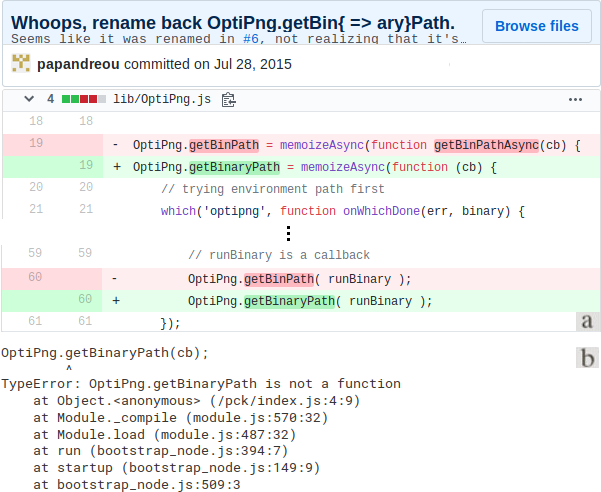
\includegraphics[scale=0.65]{figuras/bc_optipng.png}
    \caption{\textit{a}: \textit{stack trace} da \textit{breaking change}. \textit{b}: \textit{commit} que corrigiu a \textit{breaking change}}
    \label{fig:bc_optipng}
\end{figure}{}